\section{Hazard Analysis and Critical Control Point (HACCP) Plan}
% Specific focus on the safety of the system's processes and food outputs

% HACCP is a systematic approach to the identification, evaluation, and control of food safety hazards. A HACCP Plan is the written document which is based upon the principles of HACCP and which delineates the procedures to be followed.
% The Teams’ HACCP Plan should follow the principles and guidelines of a HACCP Plan as described by the U.S. National Advisory Committee on Microbiological Criteria for Foods (NACMCF) and the associated prerequisite programs (where applicable).
% The Basic HACCP Plan desired at this Progress Report stage (May 31 deadline) is only expected to be a starting point for the final Basic HACCP Plan expected to be a part of the final report (due in January 2023).

% Def'n of terms: https://www.fda.gov/food/hazard-analysis-critical-control-point-haccp/haccp-principles-application-guidelines#princ
% HACCP reference: https://spinoff.nasa.gov/moon-landing-food-safety?utm_source=TWITTER&utm_medium=KathyLueders&utm_campaign=NASASocial&linkId=141839394

\subsection{Food Production System Description}
% Incl. flowchart

% PeaPod uses automated control systems to generate desired environments. These are air thermoregulation, humidity control, LED lighting, and an aeroponics system. They are automated by an onboard computer and housed in a "control module" at the top of the unit. This lets power be "multiplied" for extended PeaPods by adding more control modules in a controller-follower topology.

% PeaPod is an automated plant growth environment, comprised of several control systems regulated by an automation and monitoring system within a modular, cubic housing. It can generate any desired environment while collecting data on plant growth and improving yields. Due to the wide range of actuation for each control system's environment parameter, and the extendable housing topology, the growth environment is adaptable to any plant or mission requirements. In addition, plant growth support platforms (with watering system) and lighting systems are built on modular "trays" mounted to the inside of the housing so the user can position plants and lights to accommodate any plant size.

% PeaPod's control systems are made of environmental controls (feedback loops with sensors) and plant inputs (set-states):
% \begin{itemize}
%     \item\textit{Lighting}: A wide spectrum of LEDs, from IR to UV, with a focus on Photosynthetically Active Radiation (PAR). Dimmable LED drivers enable precision spectrum and intensity control. Efficient, precise emission spectrum, low heat.
%     \item \textit{Aeroponics}: Reverse osmosis (RO) water is pressurized by a pump (with sensor for safety cutoff), brought to temperature, nutrient-dosed and pH-balanced by custom peristaltic pumps (allows for accurate dosing, and prevents backflow under pressure), and forced through nozzles to generate mist. Root zone air temperature is regulated in the same way as the leaf zone system. Exceptions include an aluminum water block (vs internal heat sink and fan) and a single temperature sensor after the block for PID feedback in a flowing system. Runoff water is recycled. Water-efficient (98\% less water use than farming), nutrient-efficient (60\% less use than farming), no pH/nutrient "feedback" loop or waste water (common in hydroponics), increased root oxygenation.
%     \item \textit{Leaf-Zone Thermoregulation}: Leaf zone air temperature is regulated by a thermoelectric heat pump. Fans blow air over heat sinks connected to either face of a Peltier tile to circulate air and dissipate heat. A Proportionate-Integral-Derivative (PID) control system is informed by temperature sensors, and controls the direction and magnitude of the heat transfer. Low complexity, high safety/reliability, easy to automate (bidirectional, precisely dimmable, PID tuning).
%     \item \textit{Humidity Regulation}: Leaf zone humidity is regulated by a dead-zone bang-bang control system informed by humidity sensors.
%     \begin{itemize}
%         \item \textit{Humidification}: RO water is supplied to a tank with a fine mesh piezoelectric disc. A controllable driver circuit oscillates the disk, producing water vapour. Easy to automate.
%         \item \textit{Dehumidification}: A dry silica gel bead cartridge is covered by servo-actuated "shutters" to control dehumidification. Fans draw humid air through a HEPA filter into the desiccant and back into the growth environment on demand. The beads change color to indicate water saturation. The crew is then notified to swap and "recharge" via evaporation in a standard oven.
%     \end{itemize}
%     \item \textit{Gas Composition Regulation and Exchange}: Oxygen and carbon dioxide levels are managed by gas exchange. Input and output ports allow fans to draw air into and out of the system. HEPA filters remove microbes and aerosols, and servo-actuated "shutters" prevent unintended exchange. Gas concentration sensors inform a bang-bang control system for port activation.
% \end{itemize}

\begin{figure}[h!]
    \centering
    \frame{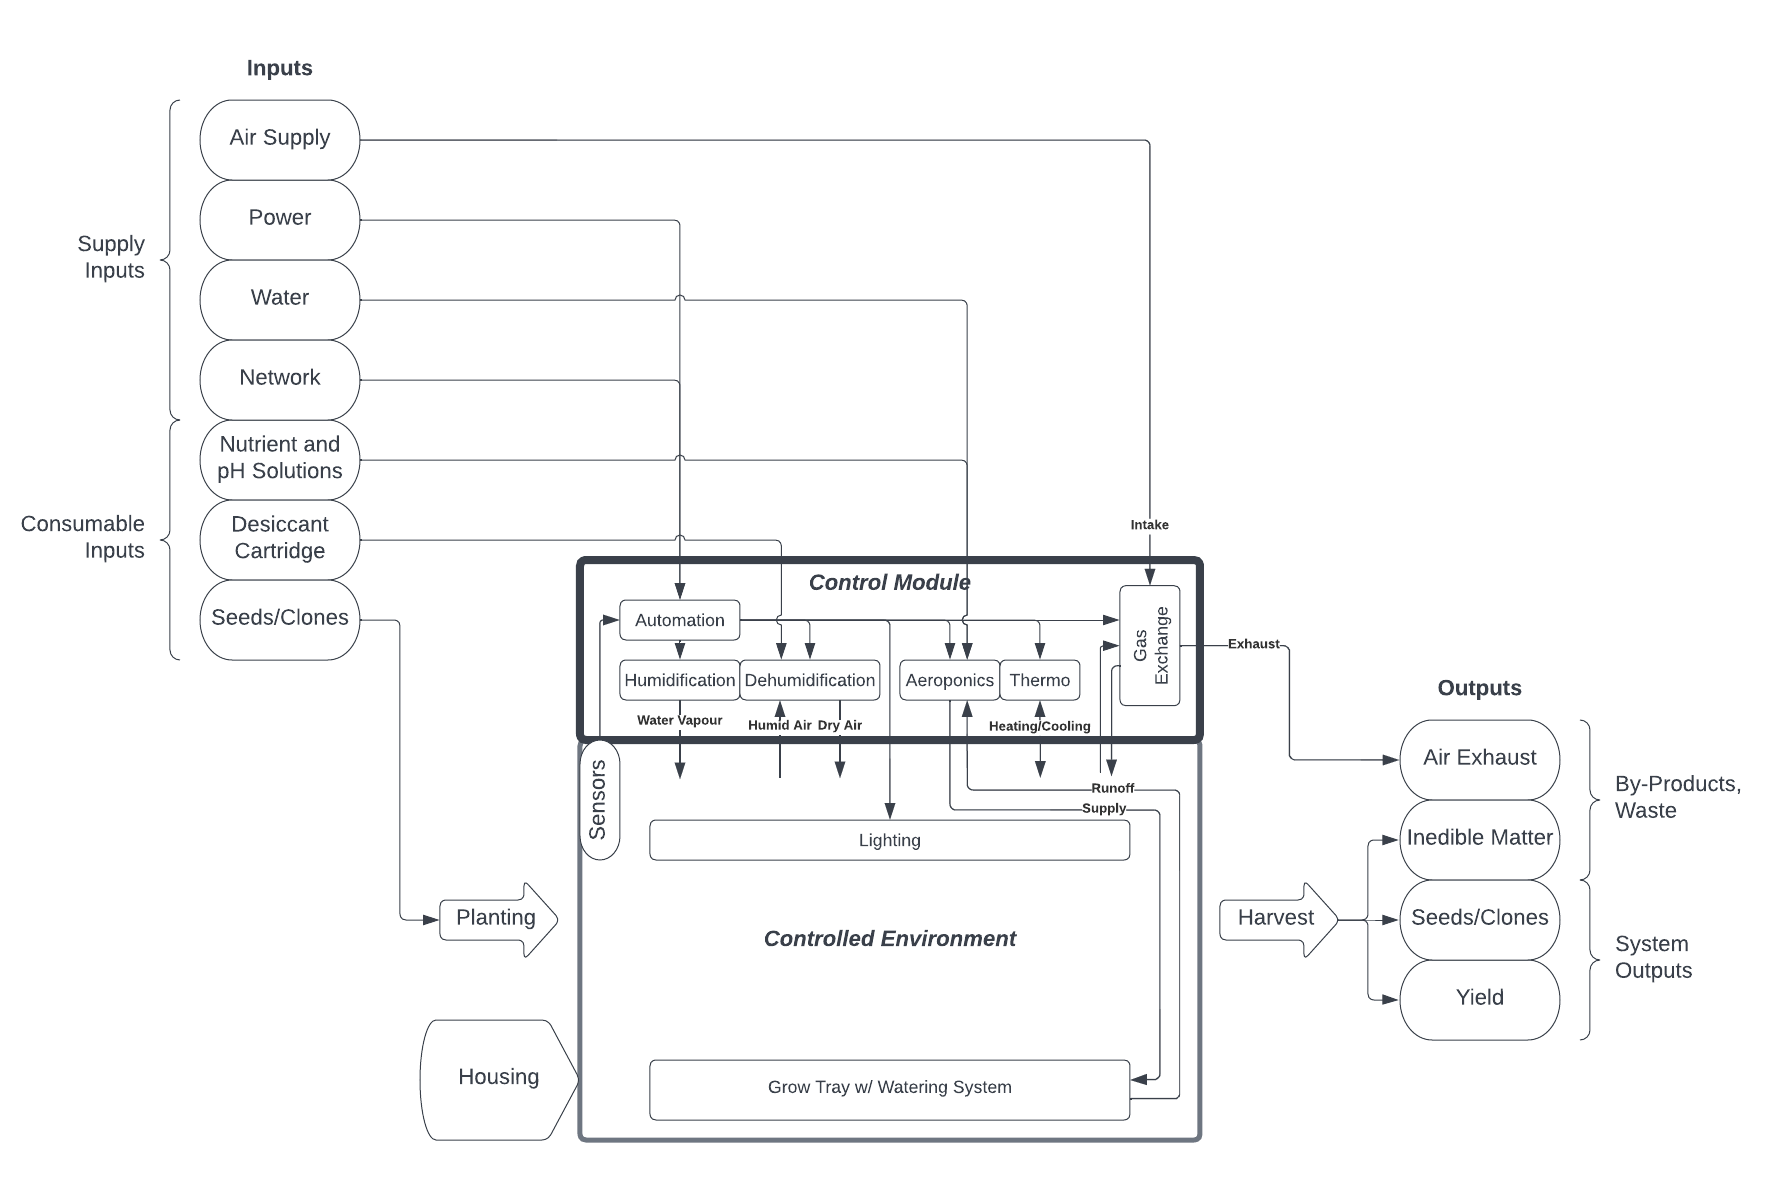
\includegraphics[width=\textwidth]{../assets/figures/system.png}}
    \caption{System overview.}
    \label{fig:system}
\end{figure}

\clearpage

\subsubsection{Hazard Analysis: Crew Contact (Harvesting, Cleaning, Maintenance)}

\begin{table}[!ht]
    \begin{tabularx}{\linewidth}{|ll|X|}
    \hline \multicolumn{2}{|l|}
        {\textbf{Source}}           & Crew contact with system during harvesting, cleaning, and maintenance  \\ \hline \multicolumn{2}{|l|}
        {\textbf{Identification}}   & Pathogens (bacteria, fungi, viruses) transferred from crew to system   \\ \hline \multicolumn{1}{|l|}{\multirow{3}{*}
        {\textbf{Evaluation}}}
        & \textit{Severity}         & Transfer of biological pathogens onto system surfaces has the potential to infect crops, posing a hazard to crew health during harvesting and ingestion. \\ \cline{2-3} \multicolumn{1}{|l|}{}
        & \textit{Likelihood}       & Fungi and viruses are of very low probability, as they cannot live on surfaces. Human gut bacteria (i.e. E. coli) is of low probability, as crew sanitation procedures are well-established. \\ \cline{2-3} \multicolumn{1}{|l|}{}
        & \textit{CCP?}             & The HACCP team determines that the risks of cross-contamination or infection are very low. Crew sanitation practices (especially prior to system interaction), practices that minimize system interaction, and sanitizing food outputs prior to consumption are adequate to control this potential hazard. \\ \hline
    \end{tabularx}
    \caption{Hazard analysis: pathogens transferred from crew to system.}
    \label{tab:hazardanalysis_systemcontact_1}
\end{table}

\begin{table}[!ht]
    \begin{tabularx}{\linewidth}{|ll|X|}
    \hline \multicolumn{2}{|l|}
        {\textbf{Source}}           & Crew contact with system during harvesting, cleaning, and maintenance \\ \hline \multicolumn{2}{|l|}
        {\textbf{Identification}}   & Pathogens (bacteria, fungi, viruses) transferred from system to crew \\ \hline \multicolumn{1}{|l|}{\multirow{3}{*}
        {\textbf{Evaluation}}}
        & \textit{Severity}         & Biological pathogens present in system materials have the potential to infect crew during interaction. \\ \cline{2-3} \multicolumn{1}{|l|}{}
        & \textit{Likelihood}       & All pathogens are of moderate probability, as they can be present in infected seeds (and thus food products at the time of ingestion). However, there are no known instances of plant-borne pathogens infecting humans. Bacteria can also be present on all surfaces. \\ \cline{2-3} \multicolumn{1}{|l|}{}
        & \textit{CCP?}             & The HACCP team determines that the risks of infection are low. However, for the sake of maximizing yield acceptability and consistency, care should be taken in seed sanitization. This, along with system sanitation practices (both pre-flight and during harvest) and practices that minimize system interaction, are adequate to control this potential hazard. \\ \hline
    \end{tabularx}
    \caption{Hazard analysis: pathogens transferred from system to crew.}
    \label{tab:hazardanalysis_systemcontact_2}
\end{table}

\clearpage

\begin{table}[!ht]
    \begin{tabularx}{\linewidth}{|ll|X|}
    \hline \multicolumn{2}{|l|}
        {\textbf{Source}}           & Crew contact with system during harvesting, cleaning, and maintenance \\ \hline \multicolumn{2}{|l|}
        {\textbf{Identification}}   & Chemical hazards to crew (i.e. heavy metals, process chemicals) introduced by system \\ \hline \multicolumn{1}{|l|}{\multirow{3}{*}
        {\textbf{Evaluation}}}
        & \textit{Severity}         & Heavy metals (i.e. lead) and chemicals introduced during manufacturing pose a threat to crew health, either during system interaction or food product ingestion. In addition, process chemicals (i.e. acidic/ basic solutions) can pose a hazard either through physical contact or accidental ingestion. \\ \cline{2-3} \multicolumn{1}{|l|}{}
        & \textit{Likelihood}       & Heavy metals are of low probability, but may be present in trace amounts in components (i.e. plumbing, electronics) and thus may come either in direct physical contact with crew(i.e. during maintenance) or be present in food products (i.e. uptake via water supply). \\ \cline{2-3} \multicolumn{1}{|l|}{}
        & \textit{CCP?}             & The HACCP team determines that the risks of heavy metal ingestion are low. All electronics, circuit boards, solder, plumbing fittings, are certified lead-free. All soldered surfaces are cleaned of flux residue. In addition, the aeroponic system is flushed of all process chemicals prior to crew interaction. Practices that include cleaning system surfaces after manufacturing, wearing gloves during handling and interaction, and cleaning food outputs of residue prior to consumption, are adequate to control this potential hazard. \\ \hline
    \end{tabularx}
    \caption{Hazard analysis: chemical hazards to system introduced by crew.}
    \label{tab:hazardanalysis_systemcontact_3}
\end{table}

\begin{table}[!ht]
    \begin{tabularx}{\linewidth}{|ll|X|}
    \hline \multicolumn{2}{|l|}
        {\textbf{Source}}           & Crew contact with system during harvesting, cleaning, and maintenance \\ \hline \multicolumn{2}{|l|}
        {\textbf{Identification}}   & Chemical hazards to system (i.e. disinfectants) introduced by crew \\ \hline \multicolumn{1}{|l|}{\multirow{3}{*}
        {\textbf{Evaluation}}}
        & \textit{Severity}         & Chemicals can remain on system surfaces, and may be present in food product, posing a hazard either through physical contact with surfaces or through ingestion. \\ \cline{2-3} \multicolumn{1}{|l|}{}
        & \textit{Likelihood}       & Disinfectants are of moderate probability. In addition, process chemicals used during maintenance (i.e. descaling agents for the aeroponics system) may be present on food product surfaces (i.e. root vegetables). \\ \cline{2-3} \multicolumn{1}{|l|}{}
        & \textit{CCP?}             & The HACCP team determines that the risks of chemical ingestion are low. Disinfectants are food-safe and dilute. In addition, the aeroponic system is flushed of all process chemicals prior to crew interaction. Practices that include wearing gloves during handling and interaction, wiping surfaces and food products with pure water prior to physical contact and ingestion, and practices that minimize system interaction are adequate to control this potential hazard. \\ \hline
    \end{tabularx}
    \caption{Hazard analysis: chemical hazards to crew introduced by system.}
    \label{tab:hazardanalysis_systemcontact_4}
\end{table}

\clearpage

\subsubsection{Hazard Analysis: Water Supply}
\begin{table}[!ht]
    \begin{tabularx}{\linewidth}{|ll|X|}
    \hline \multicolumn{2}{|l|}
        {\textbf{Source}}           & Water supply as a medium for accumulation and distribution of hazards \\ \hline \multicolumn{2}{|l|}
        {\textbf{Identification}}   & Chemical hazards (i.e. heavy metals, process chemicals) build up in water supply and transfer to produce and, in turn, crew  \\ \hline \multicolumn{1}{|l|}{\multirow{3}{*}
        {\textbf{Evaluation}}}
        & \textit{Severity}         & Heavy metals (i.e. lead) and chemicals introduced during manufacturing and process pose a threat to crew health when ingested via food product ingestion. In addition, buildup can compromise other systems (i.e. flow rate) and reduce resistance to other threats. \\ \cline{2-3} \multicolumn{1}{|l|}{}
        & \textit{Likelihood}       & Heavy metals are of low probability, but may be present in trace amounts in components (i.e. plumbing, electronics) and thus may be present in water supply for periods of time. However, regular flushing and cleansing of the supply will provide an upper bound on possible concentrations both in the supply and in any given produce. \\ \cline{2-3} \multicolumn{1}{|l|}{}
        & \textit{CCP?}             & The HACCP team determines that the risks of chemical accumulation are low. All electronics, circuit boards, solder, plumbing fittings, are certified lead-free. All soldered surfaces are cleaned of flux residue. In addition, the aeroponic system is flushed of all process chemicals prior to crew interaction. Practices that include cleaning system surfaces after manufacturing, wearing gloves during handling and interaction, and cleaning food outputs of residue prior to consumption, are adequate to control this potential hazard. \\ \hline
    \end{tabularx}
    \caption{Hazard analysis: chemical hazards accumulate in water system.}
    \label{tab:hazardanalysis_watersupply_1}
\end{table}

\begin{table}[!ht]
    \begin{tabularx}{\linewidth}{|ll|X|}
    \hline \multicolumn{2}{|l|}
        {\textbf{Source}}           & Water supply as a medium for accumulation and distribution of hazards \\ \hline \multicolumn{2}{|l|}
        {\textbf{Identification}}   & Bacteria present in water supply thrive, transfer to produce and, in turn, crew\\ \hline \multicolumn{1}{|l|}{\multirow{3}{*}
        {\textbf{Evaluation}}}
        & \textit{Severity}         & Bacteria in/on produce, surfaces, or suspended in mist can infect crew.  \\ \cline{2-3} \multicolumn{1}{|l|}{}
        & \textit{Likelihood}       & Probability of human-borne bacteria (i.e. \textit{E. coli}) is unlikely given stringent crew sanitation procedures. Other sources are infected seeds, however there are no known instances of plant-borne pathogens infecting humans. \\ \cline{2-3} \multicolumn{1}{|l|}{}
        & \textit{CCP?}             & The HACCP team determines that the risks of bacteria accumulation are low. Practices that include cleaning system surfaces after interaction, wearing gloves during handling, and flushing the water system regularly are adequate to control this potential hazard. \\ \hline
    \end{tabularx}
    \caption{Hazard analysis: bacteria grow in water system.}
    \label{tab:hazardanalysis_watersupply_2}
\end{table}

\clearpage
\subsubsection{Hazard Analysis: Nutrient Supply}
\begin{table}[!ht]
    \begin{tabularx}{\linewidth}{|ll|X|}
    \hline \multicolumn{2}{|l|}
        {\textbf{Source}}           & Nutrient Supply as a medium for accumulation and distribution of hazards \\ \hline \multicolumn{2}{|l|}
        {\textbf{Identification}}   & Bacteria in nutrient supply thrive, transfer to water and, in turn, crew  \\ \hline \multicolumn{1}{|l|}{\multirow{3}{*}
        {\textbf{Evaluation}}}
        & \textit{Severity}         & Bacteria from nutrient supply can be distributed throughout the system and infect crew. \\ \cline{2-3} \multicolumn{1}{|l|}{}
        & \textit{Likelihood}       & Nutrient supply is kept in pre-sealed packets of individual doses, meaning control on earth will eliminate introduction of threats via nutrient supply. Once in use, any bacteria will have come from the system, so presence in the nutrient supply is non-additive. \\ \cline{2-3} \multicolumn{1}{|l|}{}
        & \textit{CCP?}             & The HACCP team determines that the risks of biological threats in the nutrient supply are low. Given proper care in pre-flight steps and standard operating procedures when interacting with nutrient supply, enough practices are in place to control this hazard. \\ \hline
    \end{tabularx}
    \caption{Hazard analysis: bacteria grow in water system.}
    \label{tab:hazardanalysis_nutrientsupply_1}
\end{table}

\clearpage

\subsubsection{Hazard Analysis: Seeds}
\begin{table}[!ht]
    \begin{tabularx}{\linewidth}{|ll|X|}
    \hline \multicolumn{2}{|l|}
        {\textbf{Source}}           & Seed supply as a medium for introduction of hazards \\ \hline \multicolumn{2}{|l|}
        {\textbf{Identification}}   & Pathogens (bacteria, fungi, viruses) present in seed supply are introduced to system  \\ \hline \multicolumn{1}{|l|}{\multirow{3}{*}
        {\textbf{Evaluation}}}
        & \textit{Severity}         & Minimal, there are no known occurences of plant-borne pathogens infecting humans.\\ \cline{2-3} \multicolumn{1}{|l|}{}
        & \textit{Likelihood}       & Moderate, however introduction of a pathogen will have occured pre-flight. But, they are sanitized and stored in isolated pouches which also minimize likelihood of bacteria on their surfaces.\\ \cline{2-3} \multicolumn{1}{|l|}{}
        & \textit{CCP?}             & The HACCP team determines that the risks of biological threats in the seed supply are low. Given proper care in pre-flight steps and standard operating procedures when planting seeds, enough practices are in place to control this minimally risky hazard. \\ \hline
    \end{tabularx}
    \caption{Hazard analysis: pathogens introduced via seed supply.}
    \label{tab:hazardanalysis_seedsupply_1}
\end{table}

\clearpage
\subsubsection{Hazard Analysis: Testing}
\begin{table}[!ht]
    \begin{tabularx}{\linewidth}{|ll|X|}
    \hline \multicolumn{2}{|l|}
        {\textbf{Source}}           & Testing as a method for propagation or introduction of threats \\ \hline \multicolumn{2}{|l|}
        {\textbf{Identification}}   & Chemical hazards (i.e. process chemicals) introduced by testing apparatus \\ \hline \multicolumn{1}{|l|}{\multirow{3}{*}
        {\textbf{Evaluation}}}
        & \textit{Severity}         & Minimal, testing substances are either buffer solution in small quantities or trace amounts of indicators on paper strips.\\ \cline{2-3} \multicolumn{1}{|l|}{}
        & \textit{Likelihood}       & Minimal, as any testing would be conducted outside of the unit using a sample collected by crew contact (see \ref{tab:hazardanalysis_systemcontact_3}, \ref{tab:hazardanalysis_systemcontact_4}).\\ \cline{2-3} \multicolumn{1}{|l|}{}
        & \textit{CCP?}             & The HACCP team determines that the risks of testing introducing chemical hazards into the system are minimal. This is given the mundane, external nature of the substances at play as well as the process design of PeaPod which intentionally limits the frequency of testing. \\ \hline
    \end{tabularx}
    \caption{Hazard analysis: chemical hazards introduced via testing.}
    \label{tab:hazardanalysis_testing_1}
\end{table}

\begin{table}[!ht]
    \begin{tabularx}{\linewidth}{|ll|X|}
    \hline \multicolumn{2}{|l|}
        {\textbf{Source}}           & Testing as a method for propagation or introduction of threats \\ \hline \multicolumn{2}{|l|}
        {\textbf{Identification}}   & Bacteria propagated by testing apparatus and procedures \\ \hline \multicolumn{1}{|l|}{\multirow{3}{*}
        {\textbf{Evaluation}}}
        & \textit{Severity}         & Severe, can inflate bacterial populations from negligible to significant, widespread, systemic threats.\\ \cline{2-3} \multicolumn{1}{|l|}{}
        & \textit{Likelihood}       & Minimal, as bacterial testing is limited if not eliminated by the process design of PeaPod and the lack of resources in the field.\\ \cline{2-3} \multicolumn{1}{|l|}{}
        & \textit{CCP?}             & The HACCP team determines that the risks of testing propagating bacterial hazards are minimal. This is given the process design of the system which avoids bacterial testing and the stringent system controls which are designed for elimination of bacteria in the first place. \\ \hline
    \end{tabularx}
    \caption{Hazard analysis: bacterial propagation induced via testing.}
    \label{tab:hazardanalysis_testing_2}
\end{table}

\clearpage

\subsection{Critical Points}

No critical points were identified in hazard analysis.
%assembly: only approved parts that have been checked for leaks, contamination, materials, air-tightness

%seeds: vetted and tested breed from an approved supplier, not opened until moment of planting, food safety steps followed while doing so (hand washing, gloves, masks, hairnet...)

%growth medium: tested for bacteria/pests, handled carefully before installation

%system inputs: filtered air, clean water, properly sourced nutrients, all tested by appropriate standards

%maintenance: plants properly isolated when non-food safe materials are present---i.e. if LED boards need to be swapped, if something needs to be greased, if something needs to be glued

%harvesting: all food safety guidelines to be followed - hand washing, gloves, masks, washing, etc.

%re-planting: checking for no old growth medium, sanitizing growth tray with food-safe sanitizer

% \subsubsection{Critical Point A}
% % Repeat for all control points

% \textbf{Hazard Description}
% % aka hazard analysis, discover CCPs

% \textbf{Critical Limits}
% % What is the safe range AND the failure conditions for the CCP

% \textbf{Monitoring Procedures}
% % How do we know the state of the CCP

% \textbf{Deviation Procedures}
% % aka corrective actions
% % How do we keep the CCP within range?

% \textbf{Associated Documents}
% record-keeping and documentation procedures

% TODO: Verification Procedures?

\subsection{Standard Test Record}
% TODO: What exactly is this?

% EXAMPLE

% Record for ingredients/materials for which critical limits have been established.
    % Supplier certification records documenting compliance of an ingredient/material with a critical limit.
    % Processor audit records verifying supplier compliance.
    % Storage records (e.g., time, temperature) for when ingredient/material storage is a CCP.

% Processing, storage and distribution records
    % Information that establishes the efficacy of a CCP to maintain product safety.
    % Data establishing the safe shelf life of the product; if age of product can affect safety.
    % Records indicating compliance with critical limits when packaging materials, labeling or sealing specifications are necessary for food safety.
    % Monitoring records.
    % Verification records.

% Deviation and corrective action records.

% Employee training records that are pertinent to CCPs and the HACCP plan.

% Documentation of the adequacy of the HACCP plan from a knowledgeable HACCP expert.

No critical points were identified in hazard analysis.

% \subsubsection{Purpose and Summary}

% \subsubsection{Safety and Quality}

% \subsubsection{Test Processes}

% \textbf{Preparation of Inputs}\\


% \textbf{Verification}\\


% \textbf{Setup, Maintenance, and Collection Protocols}\\


% \textbf{Storage}\\


% \textbf{Cleanup and Turnover}\\


% \subsubsection{Closeout}

